\chapter{Polynomials}
\label{ch:polynomials}

\chapquote{It is India that gave us the ingenious method of expressing all numbers by means of ten symbols, each symbol receiving a value of position as well as an absolute value; a profound and important idea which appears so simple to us now that we ignore its true merit.}{Pierre-Simon Laplace, French mathematician}

Don't be scared by the complicated-sounding name: we have actually been working with polynomials throughout the course! In this chapter, we will put some new names on some old concepts, and extend those ideas into a more general form. Then we'll start with the foundations and learn the rules for performing the standard operations with polynomials: adding, subtracting, multiplying, dividing, factoring, and raising to a power.

\section{Building Polynomials}

\begin{boxexplore}[What qualifies?]
Before reading he official definition of a polynomial, consider the two lists below.

\begin{center}
\begin{tabular}{C{3cm}|C{3cm}}
\text{Polynomials} & \text{Not Polynomials}\\\hline
2x+4 & 2^x+4\\
3x & \sqrt{3x}\\
1.2y^2 & 1.2y^{-2}\\
5x^2 + 3x - 7 & \abs{5x+3}-7\\
-2w^3 - 8w^2 + w & -2w^3 - 8x^2 + y\\
\frac{1}{4}x +15 & \frac{4}{x} + 15
\end{tabular}
\end{center}

Based on this information, conjecture about what it means to be a polynomial. Which of the following (if any) are polynomials?
\[6x - 8 + 7x^{-1} \qquad\qquad 150 \qquad\qquad x^2 + x^4 - 3x^3 + 8 - x\]
\end{boxexplore}

Recall that a \gls{term} is a number, a variable, or the product (or quotient) of numbers and variables. The following expressions are all terms:
\[4 \qquad 3x \qquad 14x^6\]
We have been dealing with terms throughout this course. We know how to \textit{combine like terms}. When we perform the distributive propoerty, we are multiplying one term with each of several terms.  

Remember that terms are separated by addition and subtraction, and that an \gls{algebraic expression} is the sum or difference of terms. An expression can be a single term all by itself: since $x$ and $0$ are both terms, $x+0$ (which is the same as $x$) is an expression.

A \gls{polynomial} is a special type of algebraic expression.

\begin{boxdef}[Polynomial]
A algebraic expression which contains only a single variable, in which the coefficients are all rational numbers, and the degree of each term is a non-negative integer.
\end{boxdef}

Recall that the \gls{degree of a term} is the exponent on the variable of a term. It is usually quite easy to identify the degree of a term: the degree of $5x^3$ is 3. Remember, though, that some special situations arise.

If we have a variable with no exponent, we imagine a phantom 1 as the exponent. So for example, the term $18x$ is of degree 1, since $18x = 18x^1$. If we have a number with no variable, we can imagine a phanom 1 of a different kind: a variable raised to the zero power. So, the term $10$ is of degree 0, since $10 = 10x^0$.

This means that a polynomial can always be written in the form
\[a_0x^0 + a_1x^1 + a_2x^2 + a_3x^3+ \dotsb +a_nx^n,\]
where this sum stops at some positive integer $n$, and in which the $a$-values (the coefficients) are rational numbers, some of which might be zero. Usually, we prefer to write a polynomial with the terms in order of decreasing degree, that is:
\[a_nx^n + \dotsb + a_3x^3 + a_2x^2 + a_1x^1 + a_0x^0\]

Not all algebraic expressions are polynomials. A polynomial may not have a variable in the exponent, so exponential functions are not polynomials. A polynomial may not include a variable raised to a non-integer exponent (so, no variables under radicals), nor a negative exponent (so, variables in a denominator). Also, the variable may not be enclosed in an absolute value expression.

Look back over the list of polynomials and non-polynomials in the startup exploration. The expressions in the list of polynomials all meet these requirements. The non-polynomials all fail on at least one point (can you identify the point of failure for each one?). Of the three expressions we are asked to classify, the first one is not a polynomial, since it includes the variable $x$ raised to a negative exponent. 

The other two expressions are polynomials. The number 150 is a polynomial since it is of the form $150x^0$. The third expression given meets the definition of a polynomial, and can be rewritten as follows:
\[x^4 - 3x^3 + x^2 - x + 8\]

\begin{boxdef}[Degree of a Polynomial]
The degree of the highest-degree term in the polynomial.
\end{boxdef}

The degree of a polynomial is the highest exponent in the polynomial. This is very important because the highest degree has the biggest impact on the value of the expression. If we were to put a ``$y=$'' in front of the polynomial to turn it into a function, the highest degree term will tell us which family it belongs in. For example, every member of the quadratic family is a polynomial of degree 2.

\begin{boxdef}[Standard form of a polynomial]
A polynomial is written in standard form if the degree of the terms decreases from left to right, and no two terms have the same degree.
\end{boxdef} 

This is probably common sense by this point in the course. Basically, standard form is simplified (like terms are combined and there are no parentheses), and in addition, we make be sure to write the terms in a ``reasonable'' order. The highest degree term comes first, then the rest follow in order of decreasing degree. A polynomial is still a polynomial otherwise, but this format makes polynomials easier to understand and communicate.


\subsection{Naming polynomials}

In the life sciences, biological classification is the practice of grouping organisims into species, and then grouping various species together into groups, and then grouping those groups together, and so on, to produce a systematic classification of living things. Such a classification is important so that biologists can then be clear when communicating to one another.

For example, there are many different types of fruit fly, and so the term ``fruit fly'' is ambiguous. In English, we make a distinction between the so-called ``common fruit fly'' and the ``Asian fruit fly''. Biologists in Korea, however, might not use these terms in the same way (is the Asian fruit fly more common in Korea than the common fruit fly?). Biologists have therefore agreed to use a different, more universal, system for describing organisms so that they can distinguish between \textit{Drosophila melanogaster} (what we call the common fruit fly) and \textit{Drosophila suzukii} (what we call the Asian fruit fly).

The Latinized names for organisms identify the genus and species. In mathematics, we classify polynomials using Latin and Greek names that identify the degree and the number of terms.

The first name is by degree, and this is related to the name you would give to that family of functions. We worked closely with two examples in this course so far. A polynomial of degree 1 is called a \textit{linear} polynomial, and a polyonmial of degree 2 is called a \textit{quadratic} polynomial.

\begin{table}
\centering
\begin{tabular}{c@{\hspace{2em}}l}
Degree & Name\\\hline
0 & Constant\\
1 & Linear\\
2 & Quadratic\\
3 & Cubic\\
4 & Quartic\\
5 & Quintic
\end{tabular}
\label{table:polydegreenames}
\caption{List of polynomial names by degree.}
\end{table}

For polynomials with degree higher than 5, we usuall say ``polynomial of degree $n$'', or ``$n$th degree polynomial''. For example $3x^8 + 4$ is an eighth degree polynomial, or a polynomial of degree 8.

When naming a polynomial, the second name tells us how many terms it has.

\begin{table}
\centering
\begin{tabular}{c@{\hspace{2em}}l}
No. Terms & Name\\\hline
1 		& Monomial\\
2 		& Binomial\\
3 		& Trinomial\\
\end{tabular}
\label{table:polytermnames}
\caption{List of polynomial names by number of terms.}
\end{table}

For polynomials with more than three terms, we say ``polynomial with $n$ terms'' or ``an $n$-term polynomial''. For example, 
\[11x^8 + x^5 + x^4 - 3x^3 + 5x^2 - 3\]
is a polynomial with 6 terms, or a 6-term polynomial.

Note that some of these prefixes are familiar. \textit{Tri-} means ``three'' (as in triangle and tricycle), and \textit{bi-} means ``two'' (as in bicycle or bisexual). There are less familiar word parts, too: \textit{Mono-} means one (a monopoly is when a single company is the only one offering a particular product or service). The suffix \textit{-nomial} means ``names'' (this is the same root as in the words nominate and denominator).

When giving the full name of a polynomial, we include both the name by degree and the name by the number of terms. Here are some examples:

\begin{table}
\centering
\begin{tabular}{>$c<$@{\hspace{2em}}l}
\text{Polynomial}		& Name\\\hline
14x^3 					& cubic monomial\\
-1.2x^2 				& quadratic monomial\\
18						& constant monomial\\
7x-2					& linear binomial\\
2x^2 - 4x + 8			& quadratic trinomial\\
3x^3 + 2x - 11			& cubic trinomial\\
x^4 + 3					& quartic binomial\\
\end{tabular}
\label{table:polynameex}
\caption{Examples of polynomial names.}
\end{table}

% % % % % % % % % % % % % % % % % % % % % % % % % % % % % % % % % % % % % % % % 
\section{Adding, subtracting, and multiplying polynomials}

\addtodoitem{Startup explorations in the polynomial operations sections?}

The first few operations with polynomials are related to things we have seen before.

\subsection{Polynomial addition and subtraction}

To add or subtract polynomials, we simply combine like terms -- nothing new here! The only change is that we might encounter more terms than before, and perhaps terms of higher degree.

\begin{boxex}
\label{ex:polyadd}
Add: $(3x^3 + x^2 + 6x - 8) + (4x^2 + 2x - 5)$

\exsoln\ To add polynomials, we simply combine like terms. Recall that to be like terms, two terms much have identical variable parts. So, in this case, the sum of these two polynomials is:
\[3x^3 + 5x^2 + 8x - 13\]
\end{boxex}

Be sure to read carefully. A common mistake in the above example is to combine the first term of each polyomial -- but that's no good, since we are adding polynomials of different degree!

\begin{boxex}
\label{ex:polysub}
Subtract: $(7x^3-3x+1)-(x^3-4x^2-2)$

\exsoln\ When subtracting we'll have to distribute the negative, so remember to check the signs. In this case, we'll have:
\begin{commwork}
(7x^3-3x + 1) - (x^3-4x^2-2)
&=& (7x^3-3x + 1) + (-x^3-\umin4x^2-\umin2)
\\
&=& (7x^3-3x + 1) + (-x^3+4x^2+2)\\
&=& 6x^3+4x^2-3x+3
\end{commwork}
\end{boxex}

The key with subtraction is to remember that every term of that second polynomial is being subtracted.

When showing your work, it is sometimes easier to keep track of everything if we set it up like ``old school'' addition or subtraction problem. To do this, we think of the degree of the term like the place value of a digit. If there is a degree missing, we can insert a term with coefficient 0. Here's how \cref{ex:polyadd} would look:

\[\begin{array}{rrcrcrcr}
	& 3x^3 		&+& x^2	&+& 6x		&-& 8\\
+	& 0x^3		&+& 4x^2	&+& 2x		&-& 5\\\hline
	& 3x^3		&+& 5x^2		&+& 8x		&-& 13
\end{array}\]

Consider putting the subtraction in parenthesis as a reminder that every term needs to be subtracted. Here's \cref{ex:polysub} presented in this format:

\[\begin{array}{rrcrcrcr}
	& 7x^3 		&+& 0x^2	&-& 3x		&+& 1\\
-	&( x^3		&-& 4x^2	&+& 0x		&-& 2)\\\hline
	& 6x^3		&+& 4x^2		&-& 3x		&+& 3
\end{array}\]


\subsection{Polynomial multiplication}

We have already studied the key ideas of polynomial multiplication, back in \cref{sec:exposumstopowers} when we learned how to raise a sum to a power. The key idea is to use the distributive property.

For example, given the task of multiplying the linear binomials $(x+1)(x+2)$, we treat the $(x+1)$ as a single entity and distribute that over the two terms of $(x+2)$.
\begin{commwork}
{\color{blue}(x+1)}(x+2)
&=& {\color{blue}(x+1)}x + {\color{blue}(x+1)}2
& distribute the $(x+1)$
\\
&=& {\color{blue}(x+1)}{\color{red}x} + {\color{blue}(x+1)}{\color{violet}2}
& identify two new distribution opportunities
\\
&=& {\color{blue}x}\cdot{\color{red}x}+{\color{blue}1}\cdot{\color{red}x} + {\color{blue}x}\cdot{\color{violet}2}+{\color{blue}1}\cdot{\color{violet}2}
& distribute twice more
\\
&=& x^2 + x  + 2x + 2
& simplify
\\
&=& x^2 + 3x + 2
& combine like terms
\end{commwork}

We can also set things up using an old school style, as we saw back then, and this representation makes the connections more clear. Consider the two multiplication problems below: one with four-digit numbers, and one with four-term polynomials.

\[
\begin{array}{rrrrr}
		&5&6&8&2\\
\times	&3&9&4&7\\\hline
\end{array}
\qquad\text{and}\qquad
\begin{array}{rrcrcrcr}
		& 5x^3 		&+& 6x^2	&+& 8x		&+& 2\\
\times	& 3x^3		&+& 9x^2	&+& 4x		&+& 7\\\hline
\end{array}
\]

The process of multiplication is the same in these two cases: in fact, if we substitute $x=10$, we have \textit{exactly the same problem}, since we can rewrite a number in expanded form using its place value, for example:
\begin{commwork}
5682	&=&  5000 + 600 + 80 + 2\\
		&=&  5\cdot1000 + 6\cdot100 + 8\cdot10 + 2\\
		&=&  5\cdot10^3 + 6\cdot10^2 + 8\cdot10^1 + 2\cdot10^0 
\end{commwork}
This last line is the same as the polynomial $5x^3+6x^2+8x+2$, evaluated at $x=10$!

In any case, each term in one polynomial will be multiplied by each term in the other polynomial. It's a pretty tedious exercise to multiply two four-digit numbers by hand, and the same goes for multiplying two cubic polynomials. So, instead, let's look at something more interesting.

\subsection{Return of the algebra tiles}

In \cref{sec:exposumstopowers} we saw a visual representation called algebra tiles. Algebra tiles can be used to represent polynomials, although they are limited to polynomials of degree 0, 1, or 2.

Recall that the basic set of tiles includes three colored tiles that represent 1, $x$, and $x^2$. To represent negative numbers, we also have tiles of the same size, all colored red.

\begin{figure}
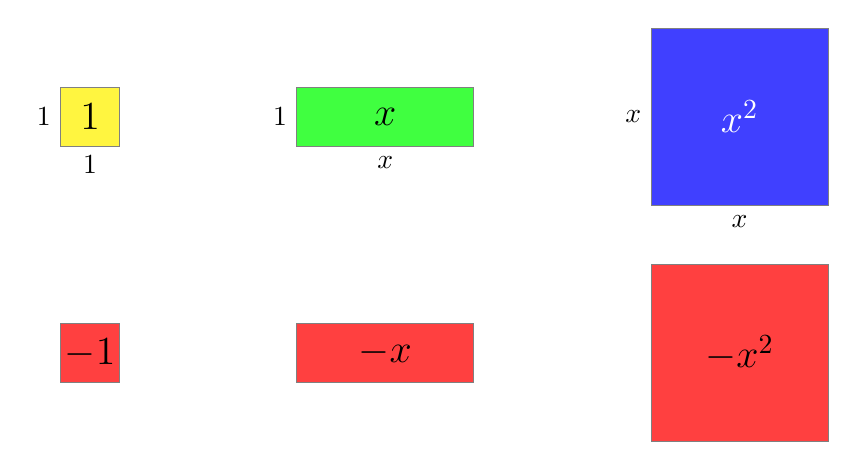
\begin{tikzpicture}[scale=0.75]
	%% 1 tile
	\draw[gray, fill=yellow!75] (0, 0) rectangle node[black]{\Large1} (1, 1);
	\draw (0.5, 0) node[below] {1};
	\draw (0, 0.5) node[left] {1};
	%% x tile
	\draw[gray, fill=green!75] (4, 0) rectangle node[black]{\Large$x$} (7, 1);
	\draw (5.5, 0) node[below] {$x$};
	\draw (4, 0.5) node[left] {1};
	%% xx tile
	\draw[gray, fill=blue!75] (10, -1) rectangle node[white]{\Large$x^2$} (13, 2);
	\draw (11.5, -1) node[below] {$x$};
	\draw (10, 0.5) node[left] {$x$};
\begin{scope}[yshift=-4cm]
	%% 1 tile
	\draw[gray, fill=red!75] (0, 0) rectangle node[black]{\Large$-1$} (1, 1);
%	\draw (0.5, 0) node[below] {1};
%	\draw (0, 0.5) node[left] {1};
	%% x tile
	\draw[gray, fill=red!75] (4, 0) rectangle node[black]{\Large$-x$} (7, 1);
%	\draw (5.5, 0) node[below] {$x$};
%	\draw (4, 0.5) node[left] {1};
	%% xx tile
	\draw[gray, fill=red!75] (10, -1) rectangle node[black]{\Large$-x^2$} (13, 2);
%	\draw (11.5, -1) node[below] {$x$};
%	\draw (10, 0.5) node[left] {$x$};
\end{scope}
\end{tikzpicture}
\end{figure}

We can use the tiles to show a picture of a polynomial, and to show how addition and subtraction work, but they are really helpful for showing the key ideas around multiplication. Let's start with the basics.

\begin{boxex}
What polynomial is represented below?

\begin{center}
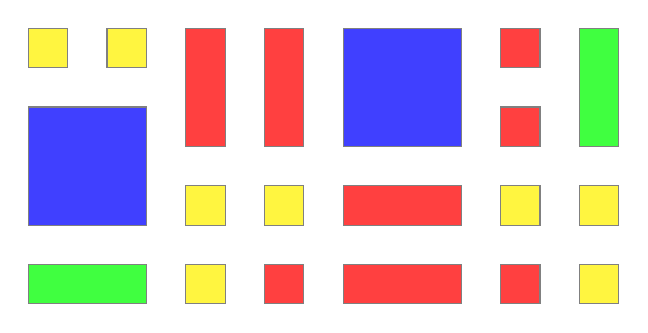
\begin{tikzpicture}[scale=0.5]
	% xx-tiles
	\foreach \x/\y/\c in {0/2/blue, 8/4/blue} {
		\draw[gray, fill=\c!75] (\x, \y) rectangle (\x+3, \y+3);
	}
	% Horiz x-tiles
	\foreach \x/\y/\c in {0/0/green, 8/0/red, 8/2/red} {
		\draw[gray, fill=\c!75] (\x, \y) rectangle (\x+3, \y+1);
	}
	% Vert x-tiles
	\foreach \x/\y/\c in {4/4/red, 6/4/red, 14/4/green} {
		\draw[gray, fill=\c!75] (\x, \y) rectangle (\x+1, \y+3);
	}
	% 1-tiles
	\foreach \x/\y/\c in {%
		0/6/yellow,%
		2/6/yellow,%
		4/0/yellow,%
		6/0/red,%
		4/2/yellow,%
		6/2/yellow,%
		12/0/red,%
		12/2/yellow,%
		12/4/red,%
		12/6/red,%
		14/0/yellow,%
		14/2/yellow%
	} {
		\draw[gray, fill=\c!75] (\x, \y) rectangle (\x+1, \y+1);
	}
\end{tikzpicture}
\end{center}

\exsoln\ A red tile will cancel out a non-red tile of the same size, since the two add up to zero. After removing all of the ``zero pairs'', we just count up what's left over. In the end, we'll have:
\[2x^2 - 2x + 4.\]
\end{boxex}

If we have two piles of tiles at the start, we can scrape them into one big pile, remove all the zero pairs, and then count up what we have. This is polynomial addition! To subtract polynomials using tiles, we would negate all the tiles in the polynomial that's being subtracted (exchanging red tiles for their non-red versions, and vice versa), and then add. Nothing to it!

Representing multiplication with algebra tiles is quite handy. The length and width are the factors and the product is the area. For instance, if we want to multply $(x+1)(x+2)$, we set up a rectangle that has width is $x+1$ and length $x+2$. We fill in the rectangle with algebra tiles and then interpret the result.

\begin{figure}
\label{fig:tileproduct}
\begin{minipage}{0.48\textwidth}
\centering
\begin{tikzpicture}[scale=0.75]
	\draw[|-|] (0,0.1) -- node[above]{$x$} (3,0.1);
	\foreach \x in {3,...,3} {
		\draw[|-|] (\x,0.1) -- node[above]{1} (\x+1,0.1);
	}
	\draw[|-|] (-0.1,0) -- node[left]{$x$} (-0.1,-3);
	\foreach \y in {-3,...,-4} {
		\draw[|-|] (-0.1,\y) -- node[left]{1} (-0.1,\y-1);
	}
	\draw[gray] (0,0) rectangle (4,-5);
\end{tikzpicture}
\end{minipage}
\begin{minipage}{0.48\textwidth}
\centering
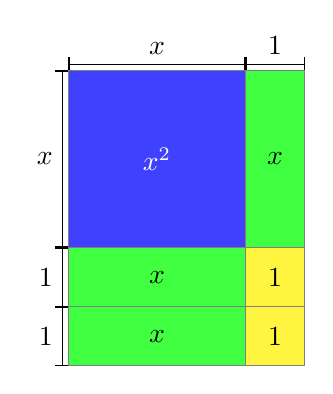
\begin{tikzpicture}[scale=0.75]
	\draw[|-|] (0,0.1) -- node[above]{$x$} (3,0.1);
	\draw[|-|] (-0.1,0) -- node[left]{$x$} (-0.1,-3);
	\draw[gray, fill=blue!75] (0,0) rectangle node[white]{$x^2$} (3,-3);
	\foreach \x in {3,...,3} {
		\draw[|-|] (\x,0.1) -- node[above]{1} (\x+1,0.1);
		\draw[gray, fill=green!75] (\x,0) rectangle node[black]{$x$} (\x+1,-3);
	}
	\foreach \y in {-3,...,-4} {
		\draw[|-|] (-0.1,\y) -- node[left]{1} (-0.1,\y-1);
		\draw[gray, fill=green!75] (0,\y) rectangle node[black]{$x$} (3,\y-1);
	}
	\foreach \x in {3,...,3} {
		\foreach \y in {-3,...,-4}
			\draw[gray, fill=yellow!75] (\x, \y) rectangle node[black]{1} (\x+1,\y-1);
	}
\end{tikzpicture}
\end{minipage}
\caption{Multiplication using algebra tiles: $(x+1)(x+2)=x^2+3x+2$}
\end{figure}

So, we have the product $(x+1)(x+2) = x^2 + 3x + 2$.

It may seem silly to manipulate these rectangular pictures one we know how to use the distributive property, but recall how helpful the square diagrams were in solving quadratic equations. Rectangular pictures will help us to visualize the ``undoing'' of multiplication in a section or two. Never underestimate the power of a picture!

\subsubsection{An algebraic {F}-word}

At this point, many algebra textbooks introduce the term \textit{FOIL}.\footnote{This term is also popular among online tutorial videos, math-help websites, private tutors, and parents.} The authors of the \algebranomicon\ are not fans of FOIL, and we mention it at this point only to dispell the misconception that we don't know what it is.

FOIL is an acronym that stands for ``First, Outer, Inner, Last''. It is meant to be a mnemonic device for remembering how to multiply two binomials.

\begin{figure}
\begin{tabular}{lll}
F & First & Multiply the first terms of the binomials\\
O & Outer & Multiply the outer terms of the binomials\\
I & Inner & Multiply the inner terms of the binomials\\
L & Last & Multiply the last terms of the binomials
\end{tabular}

\vspace{3ex}

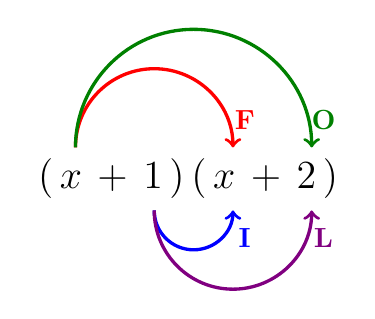
\begin{tikzpicture}
	\draw (0,0) node[right] {\Large$(\,x\,+\,1\,)\,(\,x\,+\,2\,)$};
	\draw[red, very thick, <-] (2.6, 0.4) arc (0 : 180 : 1);
	\draw (2.75, 0.75) node[red] {\textbf F};
	\draw[green!50!black, very thick, <-] (3.6, 0.4) arc (0 : 180 : 1.5);
	\draw (3.75, 0.75) node[green!50!black] {\textbf O};
	\draw[blue, very thick, <-] (2.6, -0.4) arc (0 : -180 : 0.5);
	\draw (2.75, -0.75) node[blue] {\textbf I};
	\draw[violet, very thick, <-] (3.6, -0.4) arc (0 : -180 : 1);
	\draw (3.75, -0.75) node[violet] {\textbf L};
\end{tikzpicture}
\end{figure}

The problem with FOIL is that it only works with \textit{two binomials}. It's a special-case formula! If we're going to learn a technique for multiplication, we should focus on a technique that works for everything: the distributive property always works. FOIL does not.

% % % % % % % % % % % % % % % % % % % % % % % % % % % % % % % % % % % % % % % % 
\section{Dividing polynomials}

Polynomials represent real numbers, and since we can divide real numbers, we can divide polynomials. We won't focus on polynomial division here -- it will be a topic of more dicsussion in Algebra 2. We discuss the idea now simply to ``complete the set'' and show how all four of the basic operations work with polynomials.

Polynomial division works just like long division of numbers. Recall from your elementary school days (or from \cref{sec:radrealnumbers}) that to do the division $643\div12$ we proceed like so:

\[
\renewcommand\arraystretch{1.1}
\begin{array}{*2r @{\hskip\arraycolsep}c@{\hskip\arraycolsep} *3r}
		&&&		~&5&3\\
\cline{3-6}
1&2		&\big)&		6&4&3\\
		&&-&		6&0&~\\
\cline{4-6}
		&&&		~&4&3\\
		&&&		-&3&6\\
\cline{5-6}
		&&&		~&~&7\\
\end{array}
\]

In the end, we can make 53 whole groups of 12 and we are left with a remainder of 7. In other words: we can't make another group of 12 because we have only 7 left over. We can express this as a fraction since we have $\frac{7}{12}$ of another group. So we have:
\[643 \div 12 = \frac{643}{12} = 53\,\frac{7}{12}\]
Generally speaking, we have:
\[\frac{\text{dividend}}{\text{divisor}} = \text{quotient}+\frac{\text{remainder}}{\text{divisor}}\]

Of course, if the remainder is zero then it means that the divisor is a factor of the dividend. Both of these situations can arise when dividing polynomials. Later, in Algebra 2, we will return to polynomial division and discover what we can learn from these remainders when they exist.

We find ourselves in a particularly powerful and important situation, though, when one polynomial is a factor of the other. This is the focus of \cref{ch:factoring}, and we will spend quite a bit of time learning the essential skills around \textit{factoring} polynomials.

Before we get into that special situation, let's look at some examples of polynomial division. Suppose we wish to divide $x^3-5x^2+4x-2$ by $x-2$.

First, we have to set up the division. We should check and make sure the polynomials completely simplified and that their terms are arranged by decreasing degree. Then, we set up the division:

\[
\renewcommand\arraystretch{1.1}
\begin{array}{*1r @{\hskip\arraycolsep}c@{\hskip\arraycolsep} *4r}
\cline{2-6}
x-2		&\big)	&x^3&-5x^2&+4x&-2\\
\end{array}
\]

To divide we look at the first term in the divisor and ask: ``What do we have to multiply that term by to get the first term in the dividend?'' In this case, we have to multiply $x$ (the first term in the divisor) by $x^2$ to get $x^3$ (the first term in the dividend). So, $x^2$ becomes the first term in the quotient.

\[
\renewcommand\arraystretch{1.1}
\begin{array}{*1r @{\hskip\arraycolsep}c@{\hskip\arraycolsep} *4r}
		&	~	&&x^2&\\
\cline{2-6}
x-2		&\big)	&x^3&-5x^2&+4x&-2\\
\end{array}
\]

Then, we follow the algorithm of long division. Multiply the entire divisor by $x^2$, line up these terms with their counterparts under the dividend and subtract. Watch out for those negative signs!

\[
\renewcommand\arraystretch{1.1}
\begin{array}{*1r @{\hskip\arraycolsep}c@{\hskip\arraycolsep} *4r}
		&	~	&&x^2&\\
\cline{2-6}
x-2		&\big)	&x^3&-5x^2&+4x&-2\\
		&-		&(x^3&-2x^2)\\
\cline{2-6}
		&		&~	&-3x^2\\
\end{array}
\]

Bring down the extra terms, and we have a new polynomial whose degree is less than the original. So, we start again with the division step and determine what we have to multiply the divisor by so that we match the leading term in the new polynomial. We can stop when the degree of the remainder is less than the degree of the divisor. Here's the full process in this case:
\[
\renewcommand\arraystretch{1.1}
\begin{array}{*1r @{\hskip\arraycolsep}c@{\hskip\arraycolsep} *4r}
		&	~	&&x^2&-3x&-2\\
\cline{2-6}
x-2		&\big)	&x^3&-5x^2&+4x&-2\\
		&-		&(x^3&-2x^2)\\
\cline{2-6}
		&		&~	&-3x^2&+4x&-2\\
		&		&-	&(-3x^2&+6x)&\\
\cline{4-6}
		&		&&	&-2x&-2\\
		&		&&-	&(-2x&+4)\\
\cline{4-6}
		&		&&		&&-6
\end{array}
\]

Therefore the quotient is $x^2-3x-2$ and the remainder is $-6$. Written in its final form, we have:
\[\frac{x^3-5x^2+4x-2}{x-2} = x^2-3x-2+\frac{-6}{x-2}\]
To check our solution, we can multiply the quotient by the divisor, then add the remainder. That should give us the dividend back again!

%A good way to practice is to take a couple of quadratic expressions that you know are factorable. Factor them. Then divide the polynomial by on of the factors and make sure the other factor is your answer. In Algebra 1, you will have to factor, at most, a quadratic by a linear.

That's a lot of alphabet soup and, as we mentioned above, we'll come back to generic polynomial division in Algebra 2. For the remainder of our time in Algebra 1, we will concern ourselves with the important situation in which one polynomial is a factor of another. Consider this final example as we make the transition.

\begin{boxex}
Divide $x^2-9$ by $x+3$.

\exsoln\ In this case, we find that there are terms ``missing'' from the dividend. So, we must add in a linear term with a zero coefficient: $0x$. Then, we can go about long division as usual:

\[
\renewcommand\arraystretch{1.1}
\begin{array}{*1r @{\hskip\arraycolsep}c@{\hskip\arraycolsep} *3r}
		&	~	&&x&-3\\
\cline{2-5}
x+3	&\big)	&x^2&+0x&-9\\
		&-		&(x^2&+3x)\\
\cline{3-5}
		&		&&-3x&-9\\
		&		&-&(-3x&-9)\\
\cline{4-5}
		&		&&&0
\end{array}
\]

No remainder means that we have found to polynomials which multiply together to produce the other:
\[(x+3)(x-3) = x^2 - 9\]
Check our solution by carrying out the multiplication of these two linear binomials. What happens?
\end{boxex}

% % % % % % % % % % % % % % % % % % % % % % % % % % % % % % % % % % % % % % % % 
\chaptersummary

In this chapter we learned the key ideas around describing and operating with polynomials. Much of this was old news: Addition and subtraction of polynomials is simply an application of combining like terms. Multiplication of polynomials, though it takes some careful bookkeeping, is just an application of the distributive property.

We also discussed a bit about polymial division, but only a bit. Generic polynomial division will return in Algebra 2. In the meantime, we will look at the important -- and surprisingly useful -- situation in which one polynomial is a factor of another. Onward!
